%!TEX TS-program = xelatex
%!TEX encoding = UTF-8 Unicode

% Load Thesis Class
\documentclass{DEIThesis}

\title{Funzionamento della rete satellitare Starlink}

\author{Matteo Galiazzo}
\studentId{2044941}

% Advisor
\advisor{Prof. Roberto Corvaja}

% If you are co-advised
\coadvisor{}
\coadvisorsUniversity{}

\university{Università di Padova}
\mastername{Ingegneria informatica}
\academicYear{2023/2024}

\begin{filecontents*}[overwrite]{\jobname.xmpdata}
    \Title{Funzionamento della rete satellitare Starlink}
    \Author{Matteo Galiazzo}
    \Language{it-IT}
    \Keywords{Ingegneria informatica\sep LaTeX}
\end{filecontents*}

\usepackage{makecell} 
% Document

\begin{document}
    % The front matter (Cover, ToC, Abstract, etc...)
    \frontmatter

    % The main content
    \mainmatter
    
    %!TEX root = ../main.tex

\chapter{Tipi di costellazioni satellitari}
\label{chp:intro}

Una costellazione di Internet via satellite è una costellazione di satelliti artificiali che forniscono servizi di Internet. In particolare, il termine si riferisce a una nuova generazione di costellazioni molto grandi (a volte indicate come megacostellazioni) che orbitano nell'orbita terrestre bassa (LEO) per fornire servizi Internet a bassa latenza e ad alta larghezza di banda (banda larga) \cite{jose_del_rosario_nsr_2018}.
% Nel 2020, il 63\% delle famiglie che vivono in zone rurali del mondo non ha accesso a Internet a causa dei requisiti infrastrutturali dei cavi sotterranei e delle torri di rete. Le costellazioni Internet via satellite offrono una soluzione a basso costo per espandere la copertura \cite{makena_young_low_2022}.
A novembre 2022, poco più del 63\% degli 8 miliardi di persone nel mondo utilizza Inetrnet, lasciando circa 3 miliardi di persone (e potenziali clienti) non connnessi.
Per colmare questo divario digitale, governi e aziende commerciali private stanno investendo in iniziative per costruire Internet a banda larga basata sullo spazio.
Se avranno successo, questi sforzi hanno il potenziale per connettere rapidamente le persone in tutto il mondo e cambiare l'ambiente spaziale stesso.
Diversi paesi stanno lanciando iniziative nazionali per stabilire costellazioni di satelliti in orbita terrestre bassa (\ac{LEO}) e catturare ampie porzioni di un mercato in crescita, liberando ampie risorse private o statali per farlo.

La competizione per fornire servizi a banda larga dai satelliti non è una novità.
Gli anni '90 hanno visto un simile boom commerciale di Internet a banda larga che ha prodotto scarso successo.
Aziende come Teledesic, Celestri, Globalstar e Iridium hanno tutte proposto grandi costellazioni di comunicazioni satellitari (SATCOM) in \ac{LEO}, ma quasi tutte sono finite in bancarotta all'inizio degli anni 2000.

Oggi la barriera all'ingresso in orbita è notevolmente diminuita poichè la tecnologia, i materiali e le capacità di lancio sono diventati più economici e più ampiamente disponibili.
La concorrenza internazionale per costruire, langiare e gestire un sistema a basso costo e bassa latenza che si estenda in tutto il mondo è feroce, poichè la domanda di servizi internet veloci e affidabili continua a crescere.

A partire dal 2022, solo un operatore, Starlink, fornisce un servizio basato su \ac{LEO} sul mercato libero.
Si stima che il mercato globale SATCOM crescerà fino a 40 miliardi di dollari entro il 2030, in gran parte guidato da iniziative basate su \ac{LEO}.

L'istituzione di una costellazione \ac{LEO}, comporta un investimento iniziale sostanziale, un know-how tecnico specializzato e la capacità di orientarsi in un panorama normativo complesso.
Con l'intensificarsi della concorrenza internazionale nelle comunicazioni \ac{LEO}, è fondamentale che il governo degli stati uniti crei un ambiente normativo abilitante (ma robusto) affinchè le imprese con sede negli Stati Uniti possano prosperare in patria e all'estero.

Il più grande concorrente degli Stati Uniti nella corsa alla connettività globale tramite banda larga satellitare è la Cina.
La Cina ha proposto una costellazione di 13000 satelliti in \ac{LEO} per soddisfare le esigenze residenziali e aziendali nel mercato cinese, nonchè nei mercati Internet sottosviluppati in tutto il mondo \cite{makena_young_low_2022}.

\section{Vantaggi della Low Earth Orbit}

I satelliti sono tipicamente lanciati in una di tre orbite: Low Earth Orbit (LEO) dai 160 ai 2'000 km, Medium Earth Orbit (MEO) dai 2000 ai 35786 km, o Geosynchronous Orbit (GEO) a 42164 km.
Ciascuna delle tre orbite ha i suoi vantaggi.
Per esempio, una costellazione in GEO può avere copertura globale con solo tre satelliti per la sua distanza dalla superficie terrestre.
La GEO è popolare per le comunicazioni per questo motivo.
Però, dato che i satelliti sono così distanti dalla Terra la latenza è molto alta.

\begin{figure}[htbp]
  \centering
  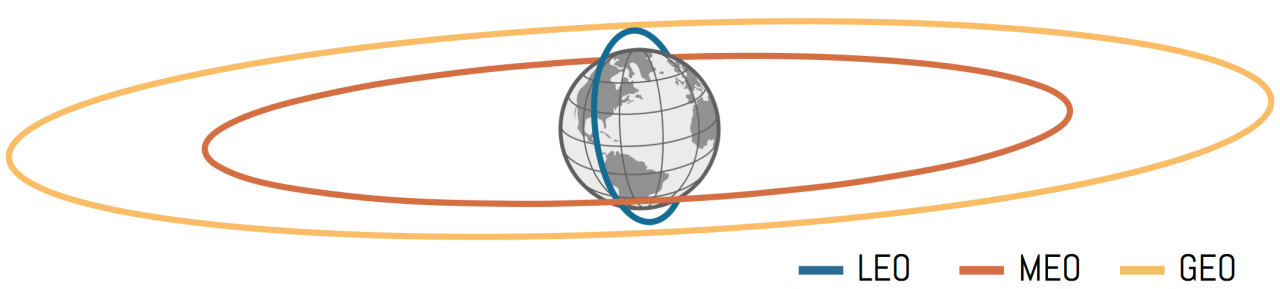
\includegraphics[width=0.9\linewidth]{./res/img/leo_orbit.png}
  \caption{Orbite terrestri di popolare utilizzo \cite{thomas_g_roberts_popular_2022}}
  \label{fig:leo-orbit}
\end{figure}

Le nuove generazioni di internet via satellite stanno collocando i satelliti in \ac{LEO} invece della tradizionale \ac{GEO} per una serie di motivi.
Infatti i satelliti lanciati in \ac{LEO} sono tipicamente più piccoli e più leggeri di quelli in \ac{GEO}, quindi serve meno carburante per mandarli in orbita e in generale sono ridotti i costi di lancio.
Inoltre, dato che i satelliti sono più vicini i terminali utente possono rilevare più satelliti allo stesso tempo e conettersi quindi al satellite più conveniente.

Le comunicazioni dalla \ac{LEO} hanno anche una latenza inferiore rispetto ai satelliti in \ac{GEO} perchè sono molto più vicini alla superficie terrestre.
Gli operatori satellitari \ac{LEO} sostengono che una pagina web può essere aperta circa otto volte più velocemente quando si utilizzano i satelliti \ac{LEO} rispetto a quando si utilizza un sistema SATCOM tradizionale in \ac{GEO}, qualcosa che è diventato più importante per i consumatori che vogliono interagire online quasi in tempo reale.
Ciò significa che Internet satellitare deve essere in grado di supportare applicazioni ad alta velocità come streaming, videoconferenza e giochi in tempo reale \cite{makena_young_low_2022}.

% https://en.wikipedia.org/wiki/SpaceX#Starlink_2
\section{Starlink}

Starlink è una costellazione internet via satellite operata da Starlink Services LLC, una consociata interamente controlla dalla società aerospaziale americana SpaceX, che fornisce copertura a oltre 100 paesi e territori.
Mira inoltre a firnire la banda larga mobile a livello mondiale.

SpaceX ha iniziato a lanciare i satelliti Starlink nel 2019.
A partire da settembre 2024, la costellazione è composta da oltre 7000 piccoli satelliti prodotti in serie in orbita terrestre bassa (\ac{LEO}) che comunicano con terminali utente sulla Terra \cite{jonathan_mcdowell_starlink_nodate}.
SpaceX prevede di schierare quasi 12000 satelliti, con una prossibile estensione successiva a 34400.
SpaceX ha annunciato di aver raggiunto più di 1 milione di abbonati nel dicembre 2022 e 4 milioni di abbonati nel settembre 2024 \cite{starlink_starlink_nodate}.

Nel maggio 2018, SpaceX ha stimato che il costo totale della progettazione, costruzione e dispiegamento della costellazione sarebbe stato di almeno 10 milardi di dollari \cite{michael_baylor_block_2018}.
Secondo quanto riferito, i ricavi di Starlink nel 2022 sono stati di 1.4 milardi di dollari, accompagnati da una perdita netta, con un piccolo profitto iniziato solo nel 2023.
Si prevede che i ricevi raggiungeranno i 6.6 milardi di dollari nel 2024 \cite{eric_berger_analyst_2024}.

Gli astronomi hanno espresso preoccupazione sull'effetto che la costellazione potrebbe avere sull'astronomia da terra e su come i satelliti contribuiranno a un ambiente orbitale già congestionato.
SpaceX ha tentato di mitigare i problemi di interferenza astronomica con misure per ridurre la luminosità dei satelliti durante il funzionamento.
I satelliti sono dotati di propulsori ad effetto Hall che consentono loro di alzare l'orbita, mantenere una posizione di stazionamento e uscire dall'orbita alla fine della loro vita.
Sono inoltre progettati per evitare collisioni in modo autonomo e senza intoppi sulla base dei dati di tracciamento collegati in uplink \cite{spacex_astronomy_2020}.
    %!TEX root = ../main.tex

\chapter{Architettura del sistema}

Chiariamo come prima cosa la differenza tra un antenna per la televisione satellitare e un'antenna Starlink.
Le parabole TV utilizzano un riflettitore parabolico per focalizzare le onde elettromagnetiche che costituiscono i segnali televisivi inviati dai satelliti di trasmissione in orbita attorno alla terra e un'altitudine di 35'000 km.
Le parabole TV ricevono solo segnali televisivi dallo spazio, non possono inviare dati.
La parabola Starlink, invece, invia e riceve dati Internet da un satellite starlink in orbita a 550km di distanza.
I fasci tra la parabola Starlink e il satellite deovno essere concentrati in fasci potenti e stretti, continuamente orientati per puntare l'uno verso l'altro \cite{branch_education_how_2022}.
Attualmente ci sono 6398 satelliti Starlink in orbita \cite{jonathan_mcdowell_starlink_nodate}.

\begin{figure}[ht]
  \centering
  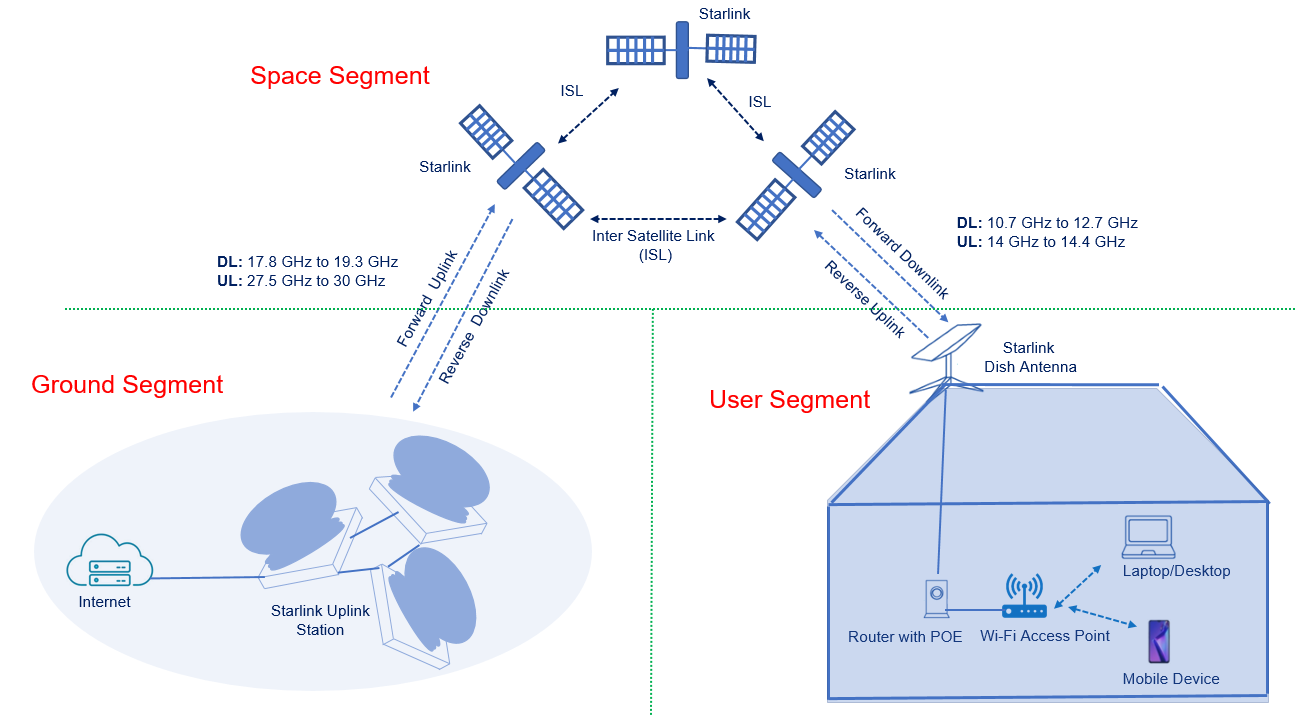
\includegraphics[width=0.9\linewidth]{./res/img/starlink-system-architecture.png}
  \caption{Architettura di sistema \cite{techplayon_spacex_2024}}
  \label{fig:starlink-system-architecture}
\end{figure}

\section{Segmento spaziale}
Questo segmento è costituito da un numero di satelliti in \ac{LEO}. Si tratta di piccoli satelliti a basso costo che pesano circa 260kg (nella versione 1.0), operano in \ac{Ku} e \ac{Ka} band e hanno durata di vita di 5-7 anni. \cite{techplayon_spacex_2024} Questi satelliti collegano l'utente a Internet.

Poichè esiste un numero enorme di satelliti questi comunicano tra loro attraverso \ac{ISL}.
% LEGGERE PAPER ISL OTTICO

\section{Segmento di terra}
I segmenti di terra includono diverse facilities che gestiscono la rete e forniscono connettività internet ai satelliti. Questi funzionano anche da Graund Station e sono localizzati strategicamente intorno al mondo per fornire copertura a zone remote e con poca connettività a internet.
La ground station è connessa all'\ac{ISP} tramite fibra.

\section{Segmento utente}
Il segmento utente comprende l'area in cui le persone utilizzano i servizi internet tramite il kit che viene fornito e che comprende l'antenna per la trasmissione, il cavo di alimentazione, il router (tranne nella versione mini dell'antenna dove il router è integrato all'antenna) e il cavo di rete per connettere l'antenna al router se quest'ultimo è incluso.

\subsection{Antenna}

\subsubsection{Struttura generale}
Aprendo la parabola (versione 1.0 revisione 2) troviamo sul retro una coppia di motori e un cavo ethernet che si collega al router.
Questi motori non muovono continuamente la parabola per puntare direttamente al satellite con cui comunica; vengono utilizzati solo durante la configurazione iniziale per orientare l'antenna nella direzione generale corretta.
Aprendo la parabola troviamo una piastra posteriore strutturale in alluminio e, dall'altro lato, una grande scheda a circuiti stampati (PCB). Su un lato ci sono 640 microchip piccoli e 20 microchip più grandi, disposti in un pattern con tracce che si diramano dai microchip più grandi a quelli più piccoli, insieme a chp aggiuntivi, inclusa la CPU principale e il modulo GPS sul bordo del PCB. Sull'altro lato cisono circa 1'400 cerchi di rame con una griglia di quadrati tra i cerchi.
Nel livello successivo c'è uno schema a nido d'ape in gomma con piccoli cerchi di rame intagliati e dietro troviamo un altro schema a nido d'ape e poi la copertura anteriore della parabola.
Abbiamo quindi 1280 antenne disposte in un pattern esagonale a nido d'ape, con ciascuna pila di cerchi di rame che rappresenta una singola antenna controllata dai microchip sul PCB.
Questo enorme array funziona insieme in quella che è chiamata un'antenna phased array per inviare e ricevere onde elettromagnetiche che vengono direzionate verso e da un satellite Starlink in orbita a 550km di distanza.

\subsubsection{Funzionamento dell'antenna Aperture Couple Patch}

\begin{figure}[htbp]
  \centering
  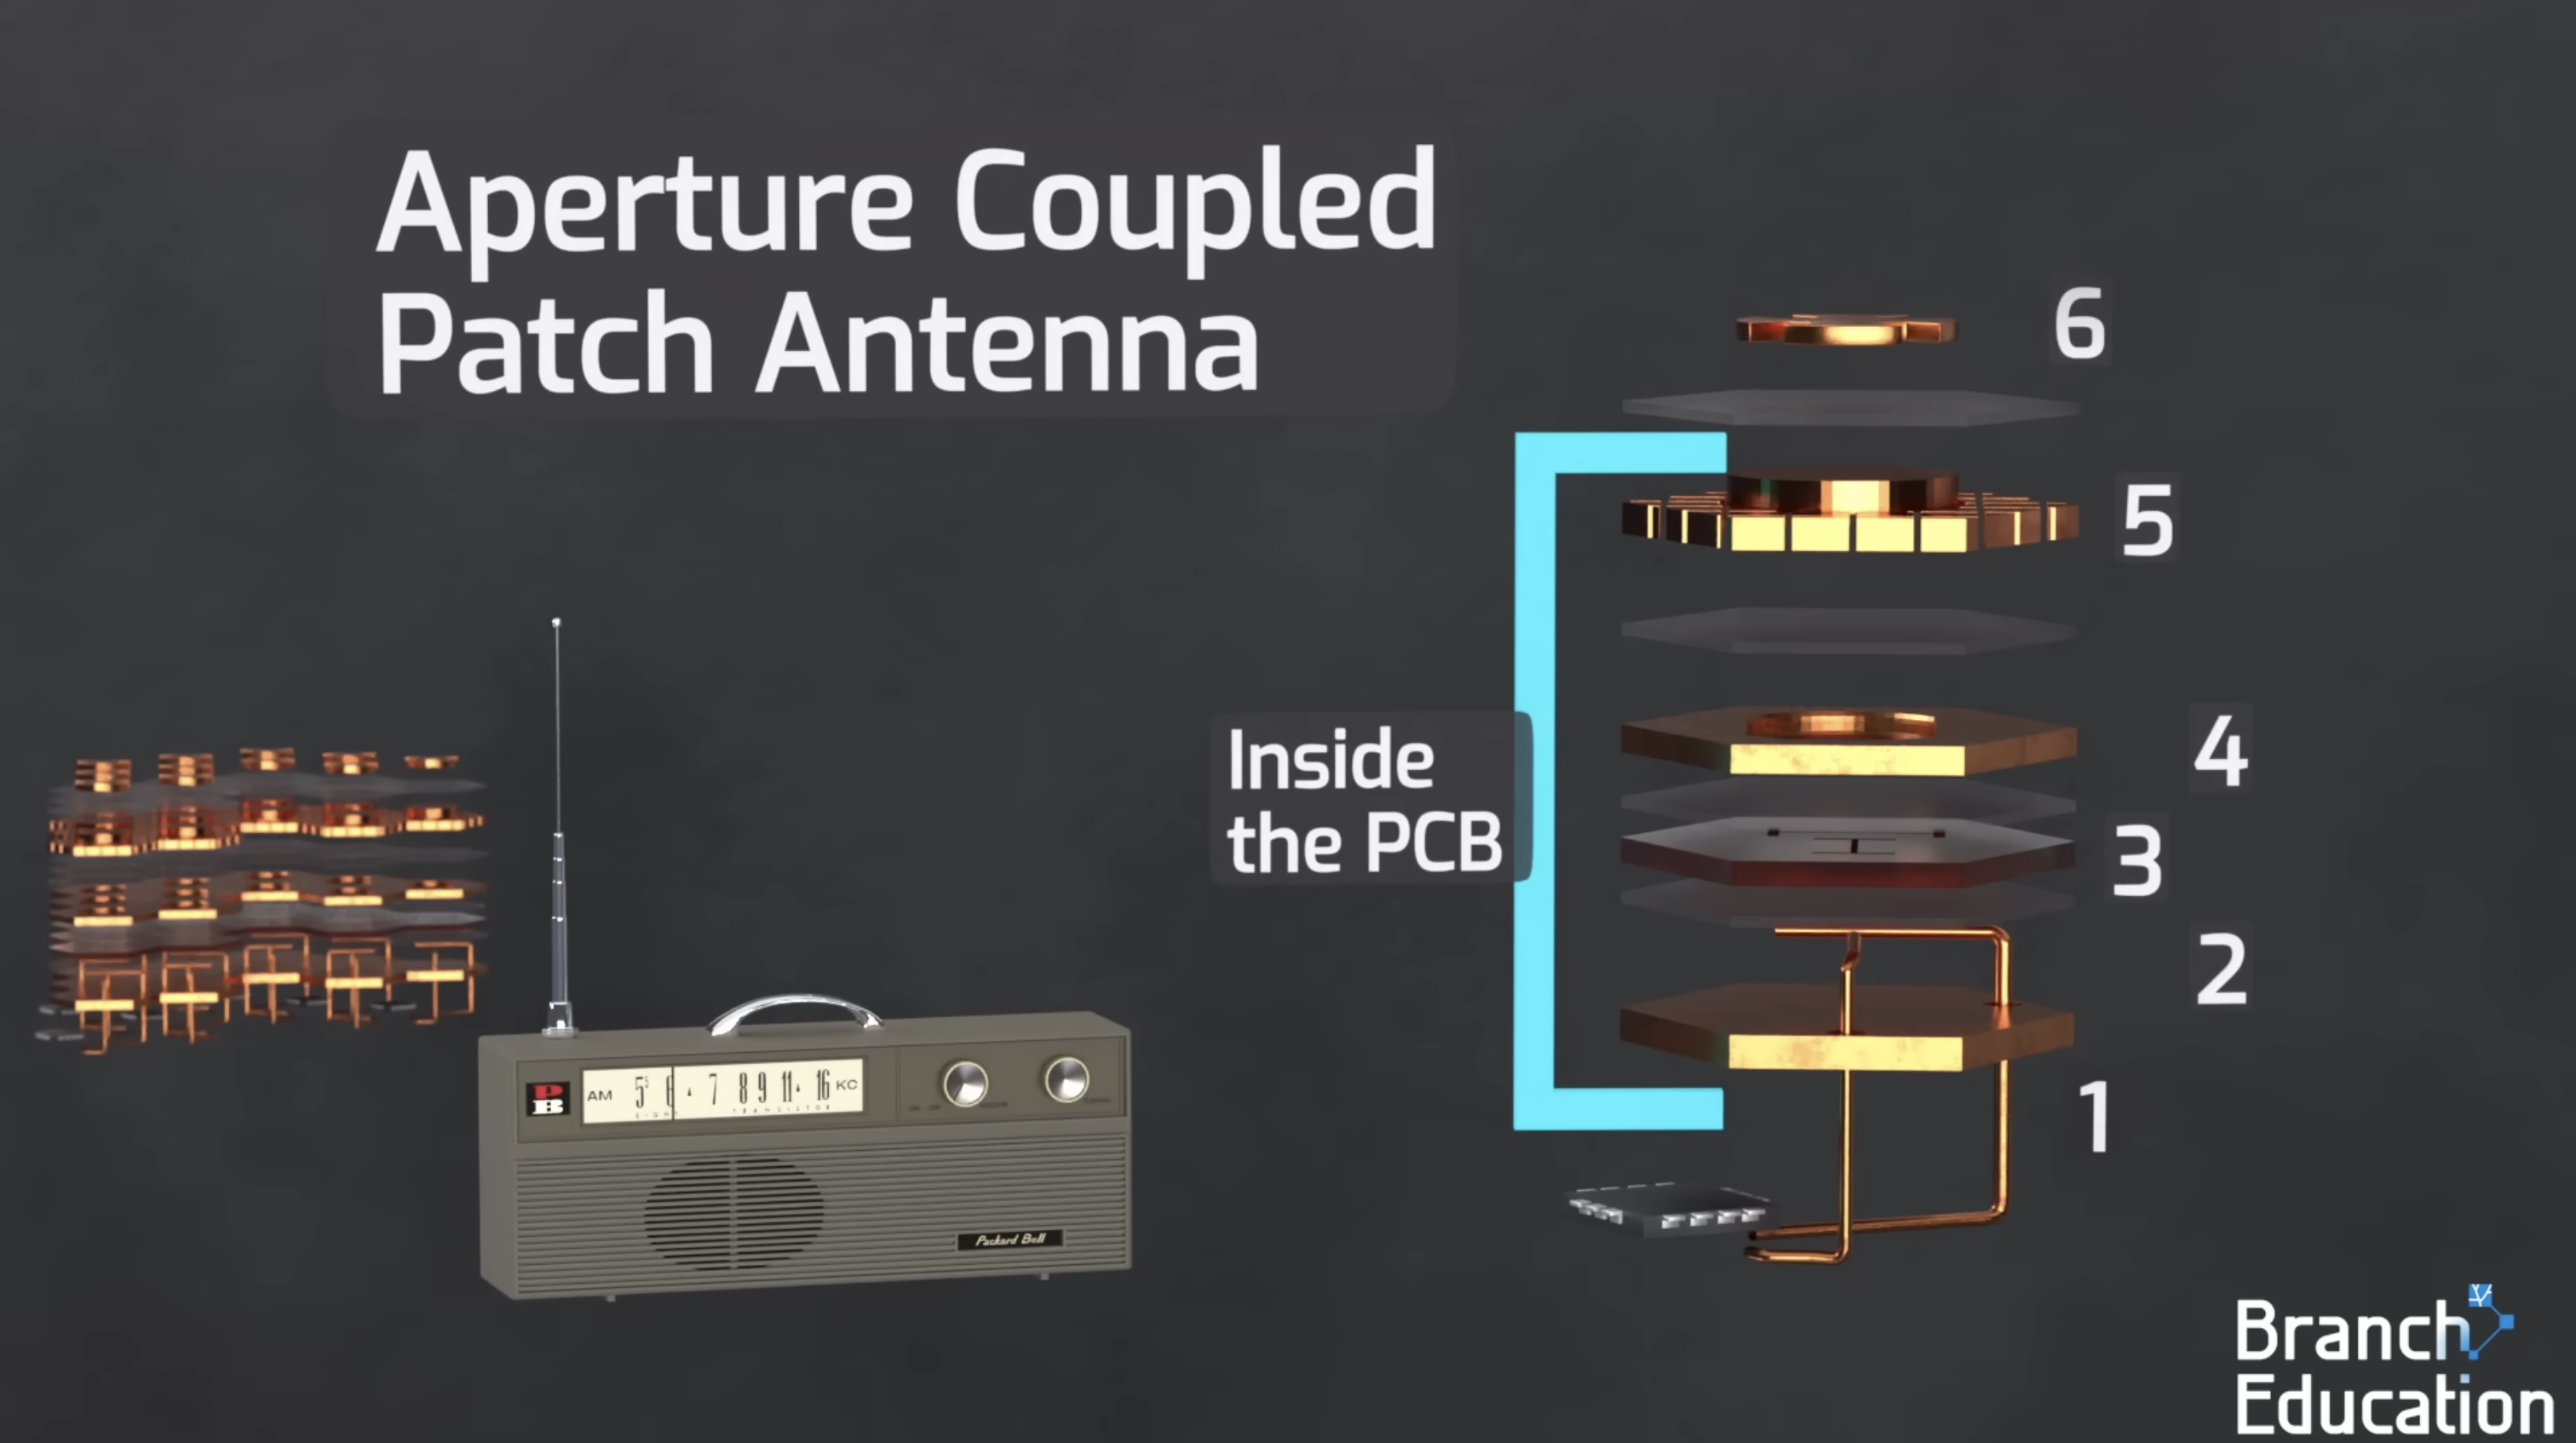
\includegraphics[width=0.8\linewidth]{./res/img/antenna_pcb.png}
  \caption{Aperture Couple Patch antenna \cite{branch_education_how_2022}}
  \label{fig:aperture-couple-patch-antenna}
\end{figure}

Nella figura \ref{fig:aperture-couple-patch-antenna} possiamo vedere un'aperture couple patch antenna, composta di 6 layer, il più dei quali all'interno del PCB.
Per semplificare la sua compressione semplifichiamola rimuovendo per il momento alcuni layer per semplificare la sua comprensione, e vediamo i principi base di come si genera un'onda elettromagnetica che si propaga da quest'antenna.

Per iniziare, sul fondo abbiamo una micro linea di trasmissione elettrica che arriva da uno dei piccoli microchip.
Questa linea di trasmissione è solo un filo di rame che termina sotto la pila dell'antenna.
Mandiamo una tensione sinusodiale alla frequenza di 12 GHz al filo di alimentazione, che vuol dire che il segnale passa da positivo a negativo ogni 83 pico secondi.
Al di sopra del filo di rame di alimentazione abbiamo un cerchio di rame con intagli chiamato patch d'antenna.

Con la corrente continua o alternata a bassa frequenza, non succederebbe molto perchè il patch è isolato, ma con un segnale ad alta frequenza la potenza inviata al filo di alimentazione viene accoppiata o inviata al patch.
Questo fenomeno avviene perchè quando la tensione è al fondo della sua sinusoide, o al minimo, c'è una concentrazione di elettroni spinti verso l'estremità del filo di alimentazione, creando così una zona di carica negativa che corrisponde alla massima tensione negativa.
Questa concentrazione di elettroni sulla punta del filo respinge tutti gli elettroni, compresi quelli sulla parte superiore del patch, e di conseguenza questi elettroni vengono spinti verso l'altro lato del patch circolare.
In questo modo, un lato del patch diventa carico positivamente, mentre l'altro diventa carico negativamente, creando così campi elettrici tra il patch e il filo di alimentazione.
Tuttavia, quando invertiamo la tensione al filo di rame 42 picosecondi dopo, abbiamo una concentrazione di cariche positive, o una mancanza di elettroni all'estremità del filo, e quindi gli elettroni nel patch fluiscono verso l'altro lato, la tensione nel patch è invertita e anche la direzione dei campi elettrici è invertita.

\begin{figure}[htbp]
  \centering
  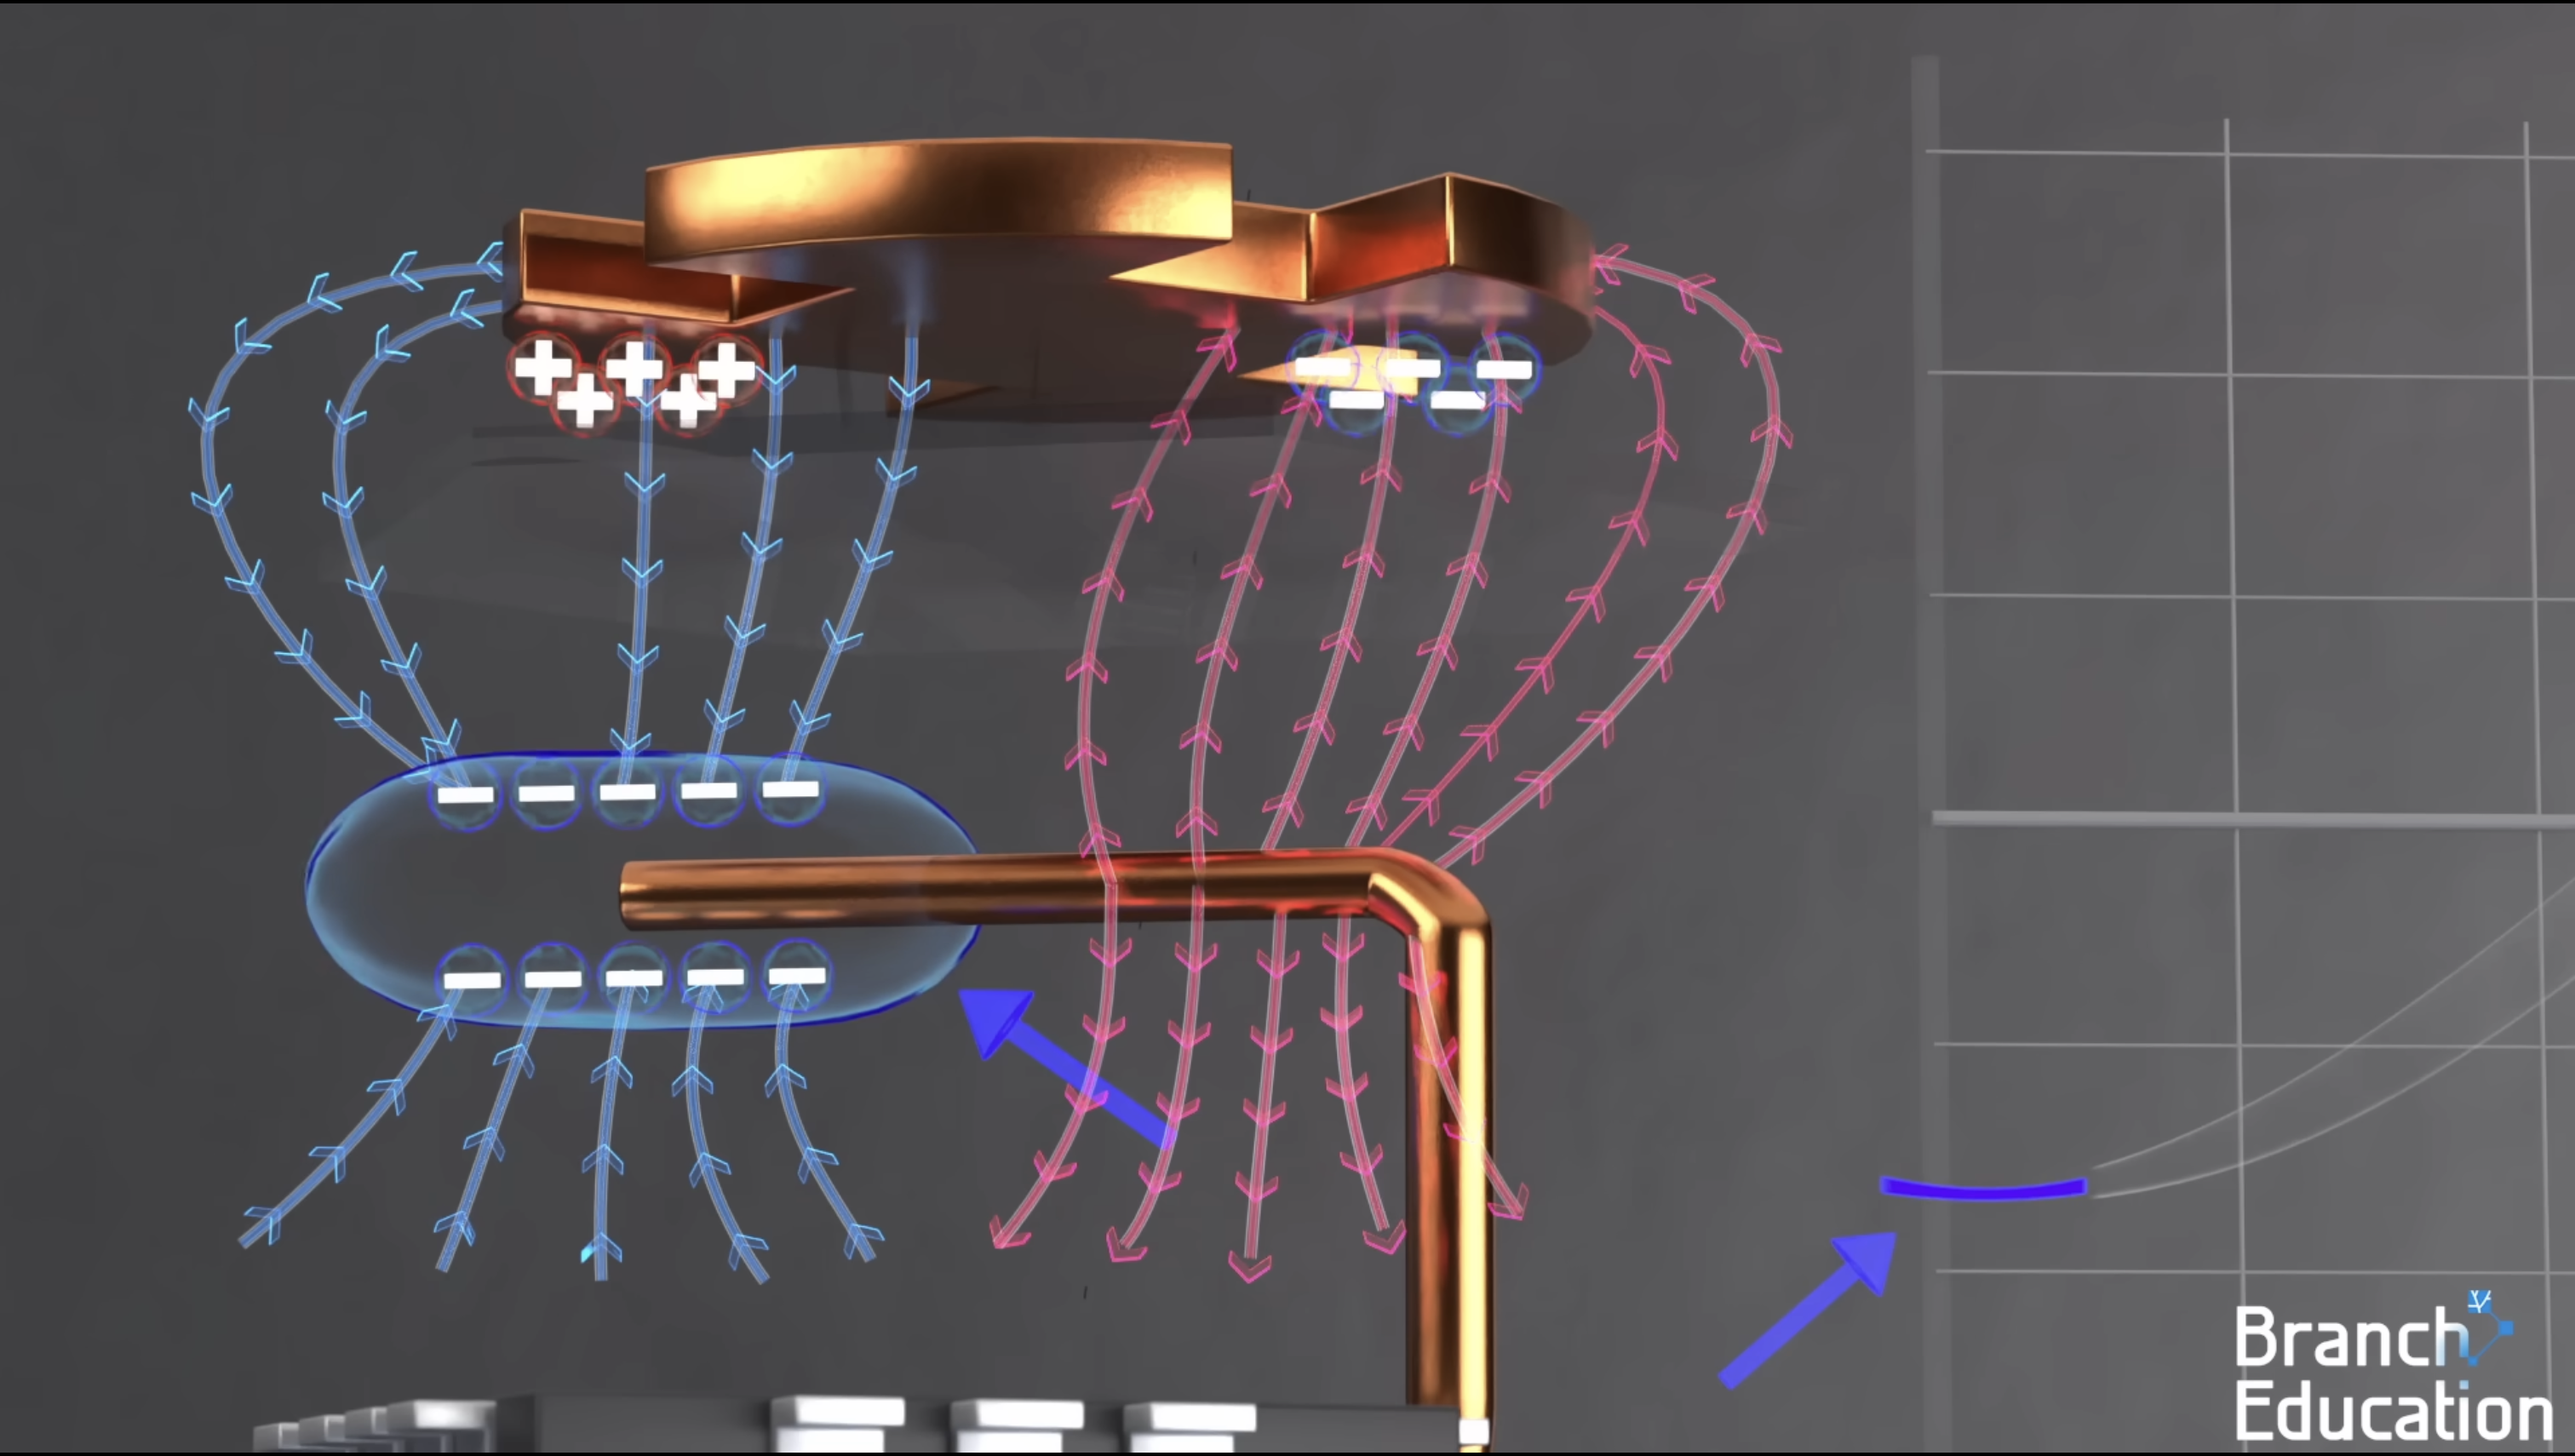
\includegraphics[width=0.8\linewidth]{./res/img/antenna_voltage_applied.png}
  \caption{Aperture Couple Patch antenna con un segnale applicato \cite{branch_education_how_2022}}
  \label{fig:aperture-couple-patch-antenna-voltage-applied}
\end{figure}

Poiché la tensione del filo di alimentazione oscilla con un intervallo di 42 picosecondi tra un picco e un avvallamento, anche i campi elettrici nel patch oscilleranno mentre gli elettroni vanno avanti e indietro.

\begin{figure}[htbp]
  \centering
  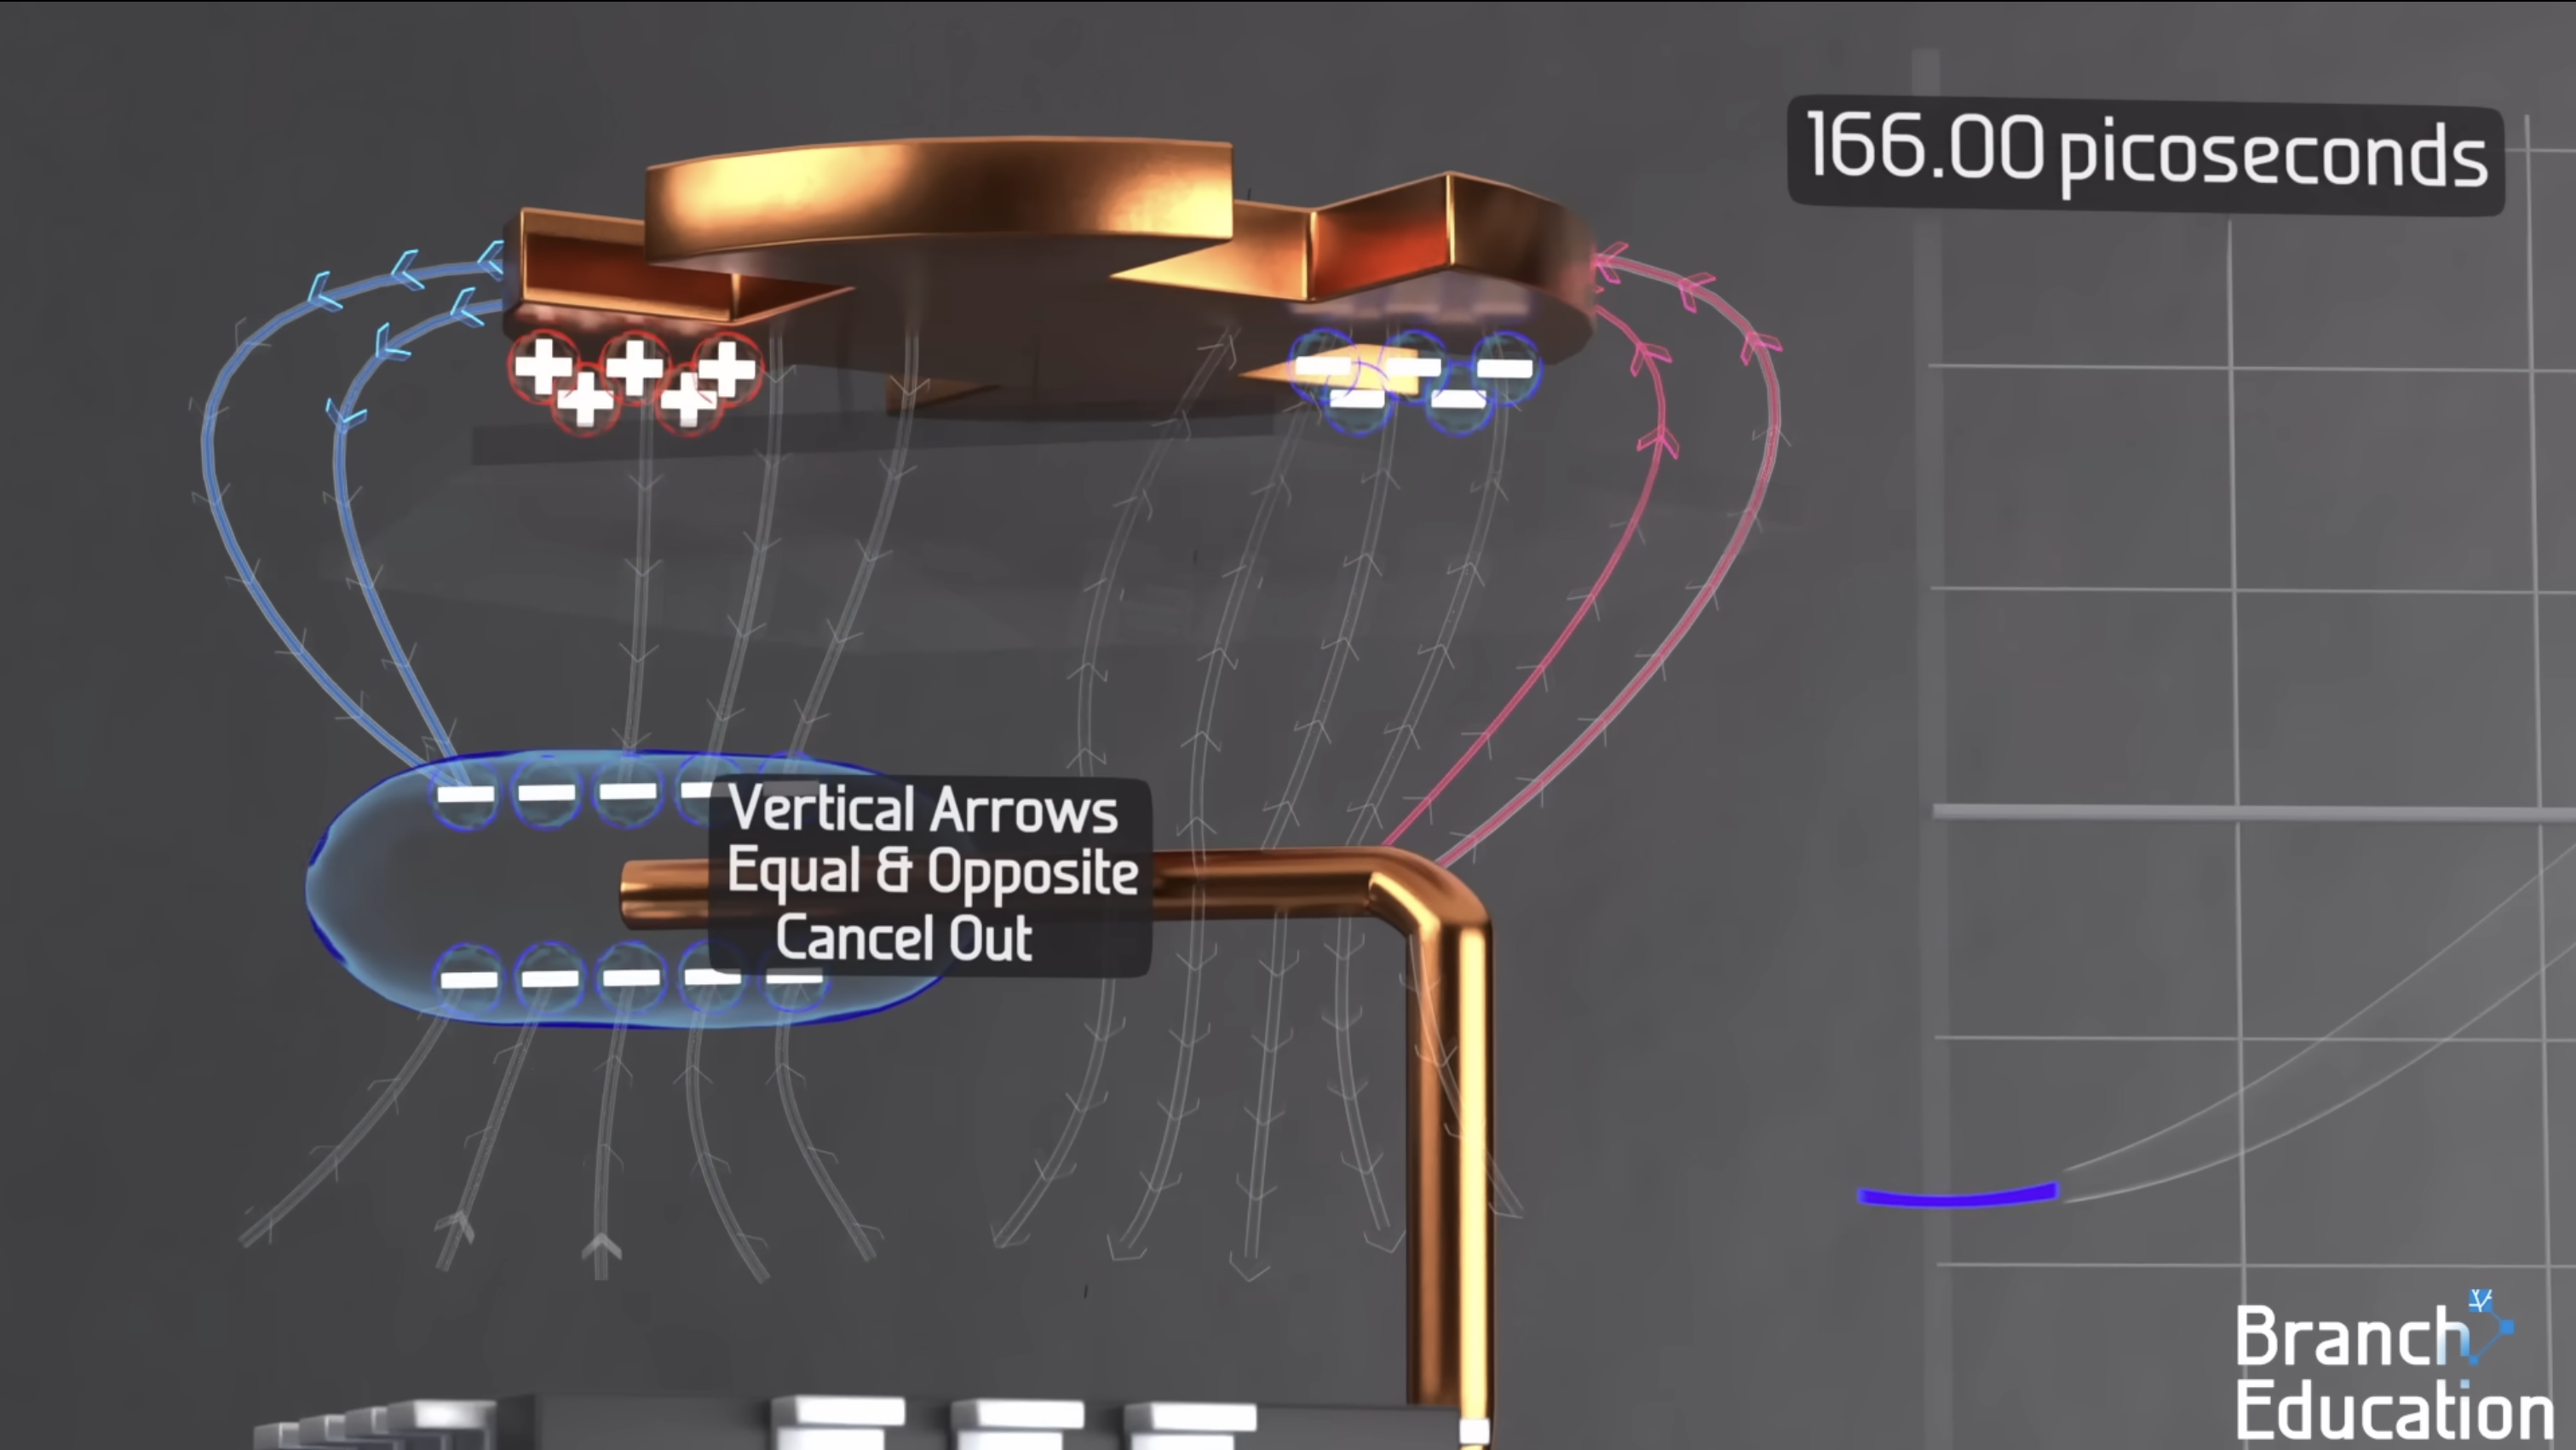
\includegraphics[width=0.8\linewidth]{./res/img/antenna_fringing_fields.png}
  \caption{Creazione dei campi di frangia in un'Aperture Couple Patch antenna \cite{branch_education_how_2022}}
  \label{fig:aperture-couple-patch-antenna-fringing-fields}
\end{figure}

Possiamo vedere in figura \ref{fig:aperture-couple-patch-antenna-fringing-fields} che alcuni di questi vettori di campo elettrico provenienti dal patch sono verticali e, poiché sono uguali e opposti, si annullano.
Tuttavia, altri campi elettrici sono orizzontali nello stesso piano del patch e sono chiamati campi di frangia.
Questi campi di frangia sono nella stessa direzione e quindi si sommano l'uno all'altro, dando luogo a un campo elettrico combinato.

Allo stesso tempo, gli elettroni che scorrono da un lato all'altro del disco, che costituiscono una corrente elettrica, generano un campo magnetico con un'intensità e una direzione, o vettore, perpendicolare al vettore del campo elettrico di frangia.
Di conseguenza, abbiamo un campo elettrico orientato in un senso e un campo magnetico orientato perpendicolarmente, come si può vedere in figura \ref{fig:aperture-couple-patch-antenna-em-field}.

\begin{figure}[htbp]
  \centering
  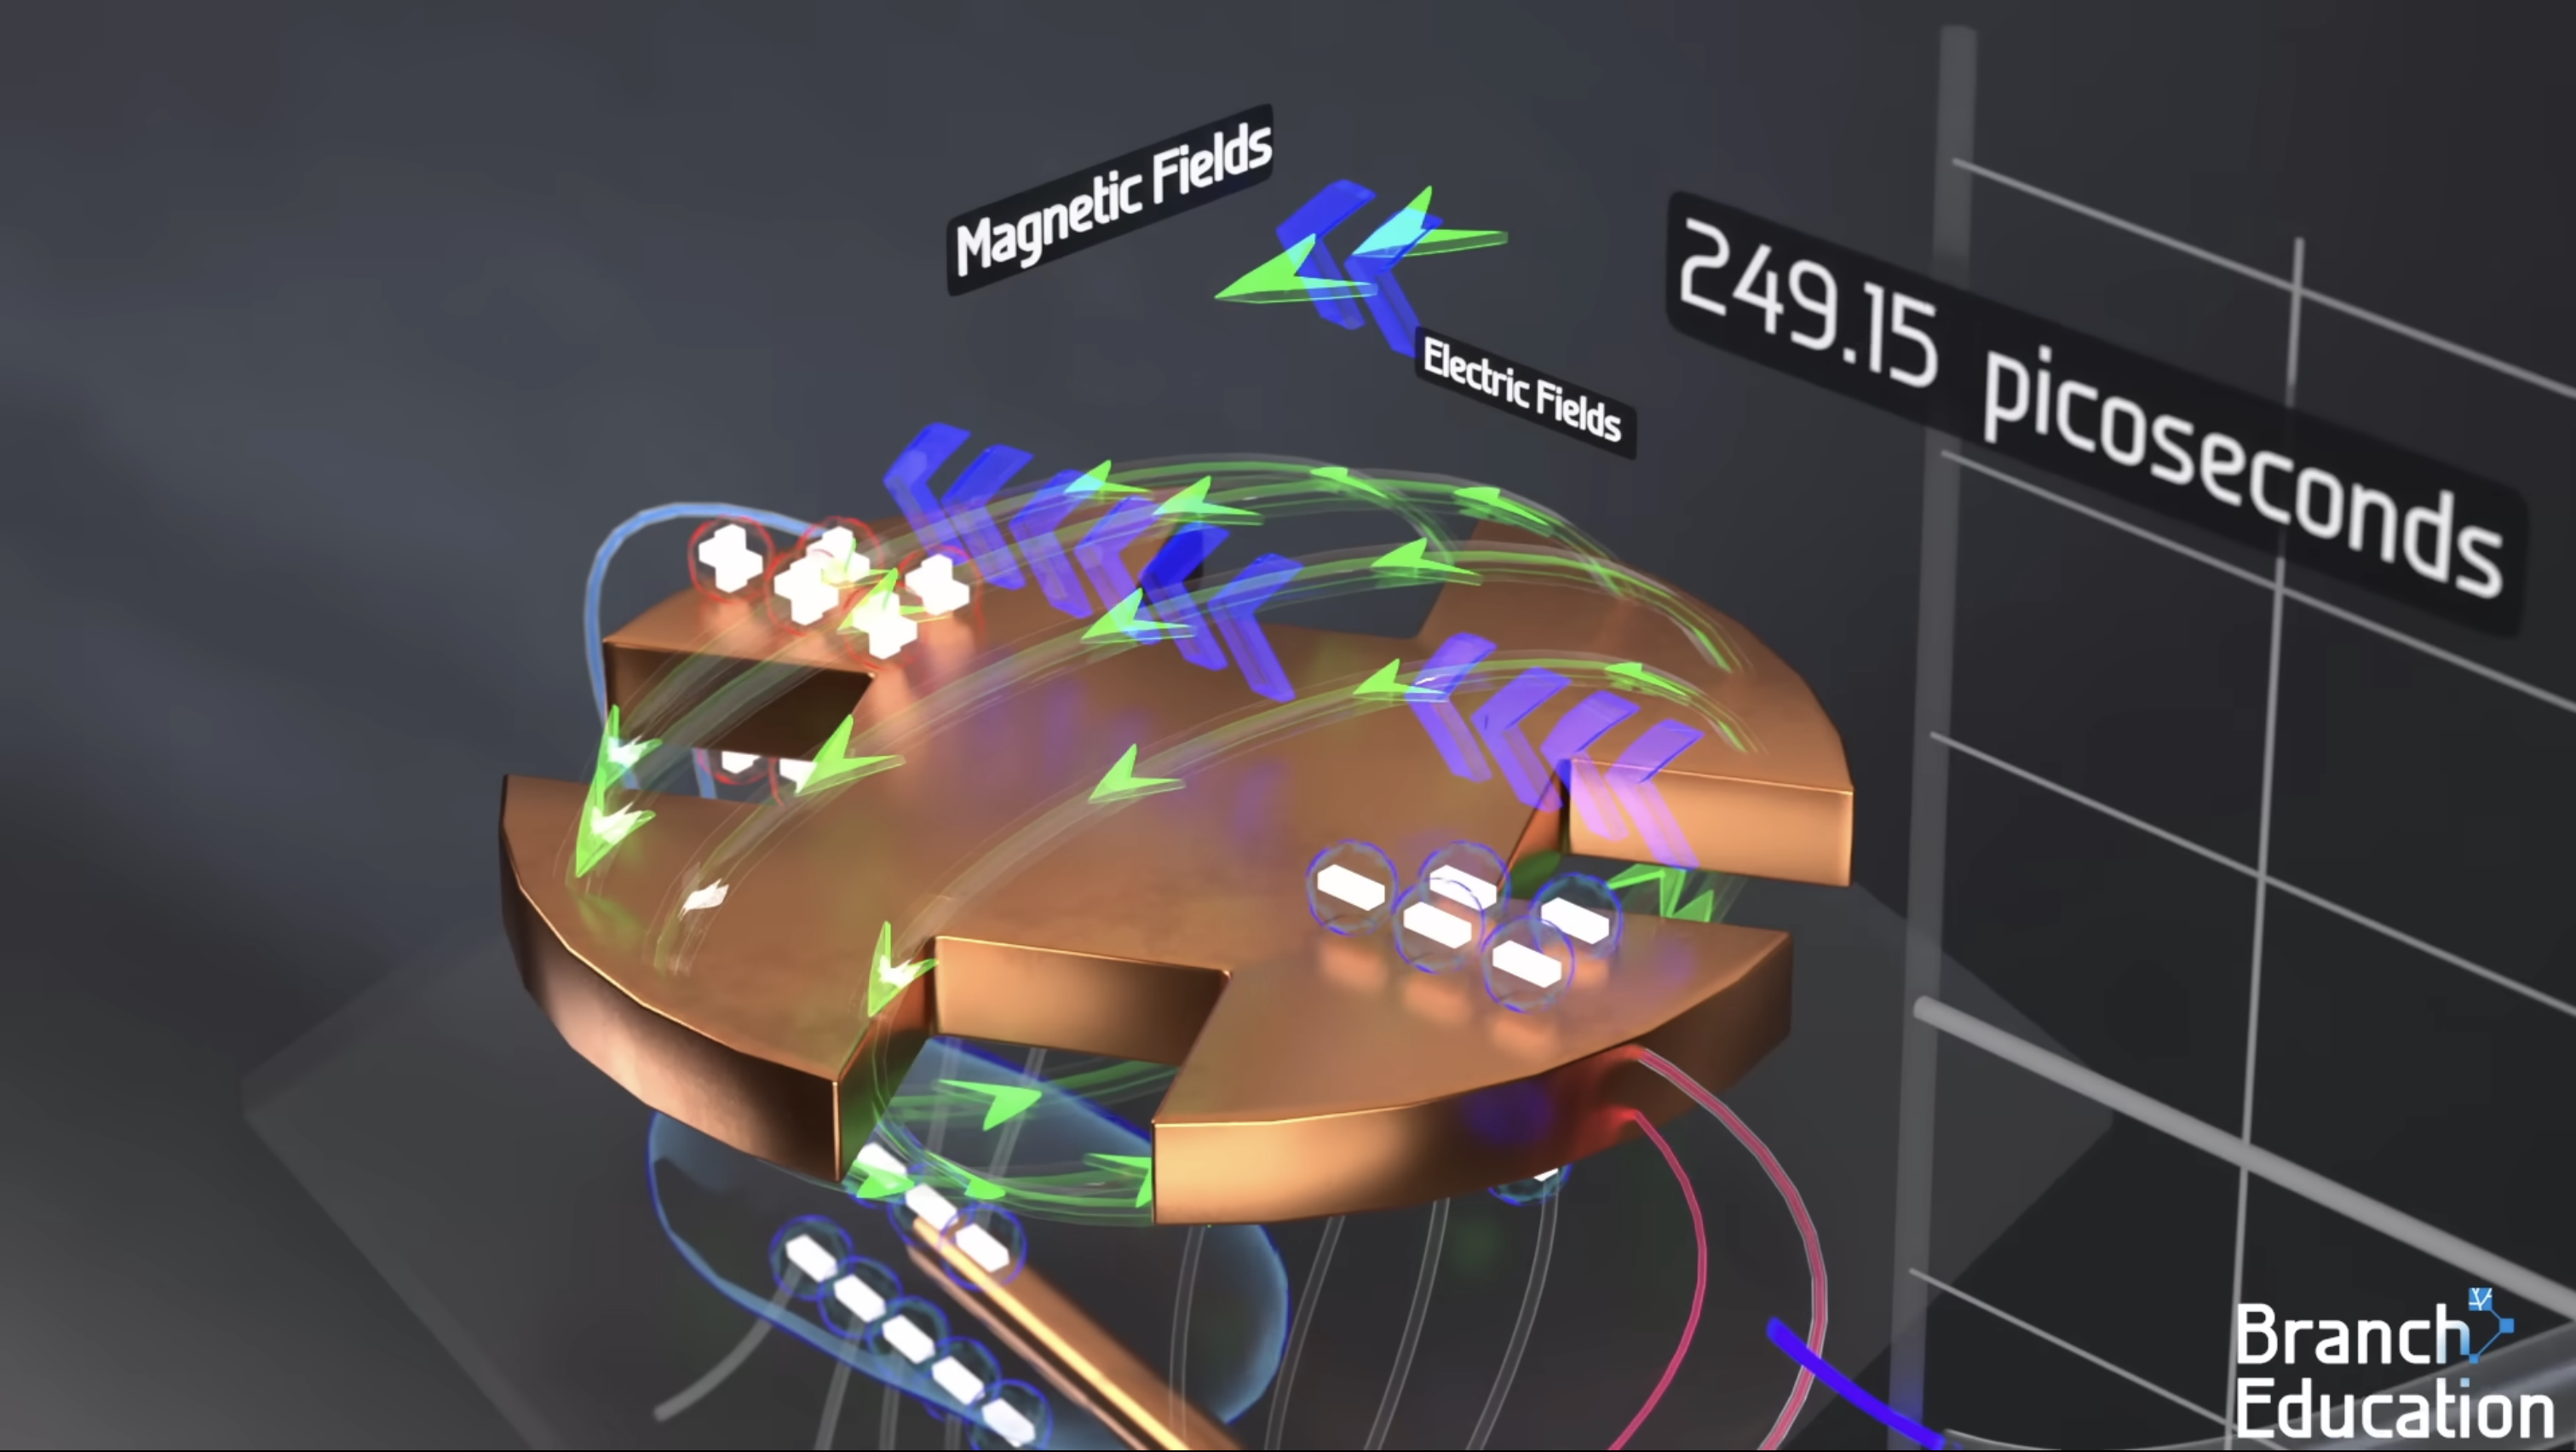
\includegraphics[width=0.8\linewidth]{./res/img/antenna_em_field.png}
  \caption{Campo elettromagnetico in un'Aperture Couple Patch antenna \cite{branch_education_how_2022}}
  \label{fig:aperture-couple-patch-antenna-em-field}
\end{figure}

42 picosecondi dopo, quando la tensione sulla linea di alimentazione diventa positiva, e siamo al picco della sinusoide, la tensione e la corrente sono invertite.
Quindi il campo elettrico e quello magnetico puntano alla direzione opposta.

\subsubsection{Emissione delle onde elettromagnetiche}
Creando i campi elettromagnetici oscillanti vengono generate onde elettromagnetiche che viaggiano in direzione perpendicolare al campo elettrico e al campo magnetico.
Dato che i due insiemi di campi vettoriali non sono tutti sullo stesso piano, ma sono curvati, l'onda elettromagnetica che si propaga viaggia verso l'esterno in una forma di guscio che si espande.

L'intensità di questi campi vettoriali è legata direttamente alla tensione che è stata originariamente mandata alla linea di alimentaizone alla base dell'antenna.

% QUI QUI QUI 10:09 video



% NUMERO DI SATELLITI, COME AVVIENE COMUNICAZIONE UTENTE-UTENTE E UTENTE-SATELLITE
    % %!TEX root = ../main.tex

\chapter{Background}
\label{chp:background}

\begin{algorithm}[ht]
    \caption{An algorithm with caption}\label{alg:two}
    \begin{algorithmic}
        \REQUIRE $n \geq 0$
        \ENSURE $y = x^n$
        
        \STATE $y \gets 1$
        \STATE $X \gets x$
        \STATE $N \gets n$
        
        \WHILE{$N \neq 0$}
            \IF{$N$ is even}
              \STATE $X \gets X \times X$
              \STATE $N \gets \frac{N}{2} $  \COMMENT{This is a comment}
            \ELSIF{$N$ is odd}
              \STATE $y \gets y \times X$
              \STATE $N \gets N - 1$
            \ENDIF
        \ENDWHILE
    \end{algorithmic}
\end{algorithm}

\begin{equation}
e^{j\pi} + 1 = 0
\end{equation}
    % %!TEX root = ../main.tex

\chapter{Analysis}
\label{chp:analysis}

\section{A section}

\tikzset{vertex style/.style={
    draw=#1,
    thick,
    fill=#1!70,
    text=white,
    ellipse,
    minimum width=2cm,
    minimum height=0.75cm,
    font=\small,
    outer sep=3pt,
  },
  text style/.style={
    sloped,
    text=black,
    font=\footnotesize,
    above
  }
}

\begin{figure}[ht]
    \centering
    \begin{tikzpicture}[node distance=2.75cm,>={Stealth[]}]
        \node[vertex style=cyan] (Rk) {Righteous Kill};
        \node[vertex style=orange, above of=Rk,xshift=2em] (BD) {Bryan Dennehy}
        edge [<-,cyan!60!blue] node[text style,above]{starring} (Rk);
    \end{tikzpicture}
    
    \caption{Image created with TikZ} \label{fig:T1}
\end{figure}

\paragraph{}
Lorem ipsum dolor sit amet, consectetur adipiscing elit, sed do eiusmod tempor incididunt ut labore et dolore magna aliqua. Ut enim ad minim veniam, quis nostrud exercitation ullamco laboris nisi ut aliquip ex ea commodo consequat. Duis aute irure dolor in reprehenderit in voluptate velit esse cillum dolore eu fugiat nulla pariatur. Excepteur sint occaecat cupidatat non proident, sunt in culpa qui officia deserunt mollit anim id est laborum.

\begin{lstlisting}[language=Python, caption=Code snippet example]
import numpy as np
    
def incmatrix(genl1,genl2):
    m = len(genl1)
    n = len(genl2)
    M = None #to become the incidence matrix
    VT = np.zeros((n*m,1), int)  #dummy variable

    test = "String"
    
    #compute the bitwise xor matrix
    M1 = bitxormatrix(genl1)
    M2 = np.triu(bitxormatrix(genl2),1) 

    for i in range(m-1):
        for j in range(i+1, m):
            [r,c] = np.where(M2 == M1[i,j])
            for k in range(len(r)):
                VT[(i)*n + r[k]] = 1;
                VT[(i)*n + c[k]] = 1;
                VT[(j)*n + r[k]] = 1;
                VT[(j)*n + c[k]] = 1;
                
                if M is None:
                    M = np.copy(VT)
                else:
                    M = np.concatenate((M, VT), 1)
                
                VT = np.zeros((n*m,1), int)
    
    return M
\end{lstlisting}
    % %!TEX root = ../main.tex

\chapter{Conclusions and Future Works}
\label{chp:conclusions}

\begin{table}[ht]
    \centering
    \begin{tabular}{|l|l|}
    \hline
    \textbf{A} & \textbf{B} \\ \hline
    C          & D          \\ \hline
    E          & F          \\ \hline
    G          & H          \\ \hline
    \end{tabular}
    \caption{Table example \label{tab:table-name}}
\end{table}
    
    % Bibliography, appendix, acknowledges, etc...
    \backmatter
\end{document}